\section{Method and Results}
\label{sec:method}

\subsection{Simulation Environment}
\label{sec:method_sim}

We developed a collection of simulation environments in Gazebo, specifically designed to replicate the layouts of typical indoor building floor plans. In addition, we have augmented the existing dragon ddk drone model with a customized ultrasonic model, enabling the simulated drone to provide simulated sonar feedback.

An example of our simulation environments is presented in Fig. \ref{fig:sim_env}, depicting an indoor building with a single loop of hallway and multiple small rooms. Along the outer walls, there are a series of empty rectangle areas representing windows. We have set the collision properties of the window material to be identical to that of the wall material. This enables us to simulate scenarios where the drone may collide with windows during navigation. Furthermore, in order to replicate the behavior of real-world depth cameras, the windows are set to be invisible to the simulated depth camera module, which is accomplished by setting the visual properties of the window material to be empty, effectively rendering the window areas transparent in depth camera images captured by the simulated drone. 

\begin{figure}[h]
    \centering
    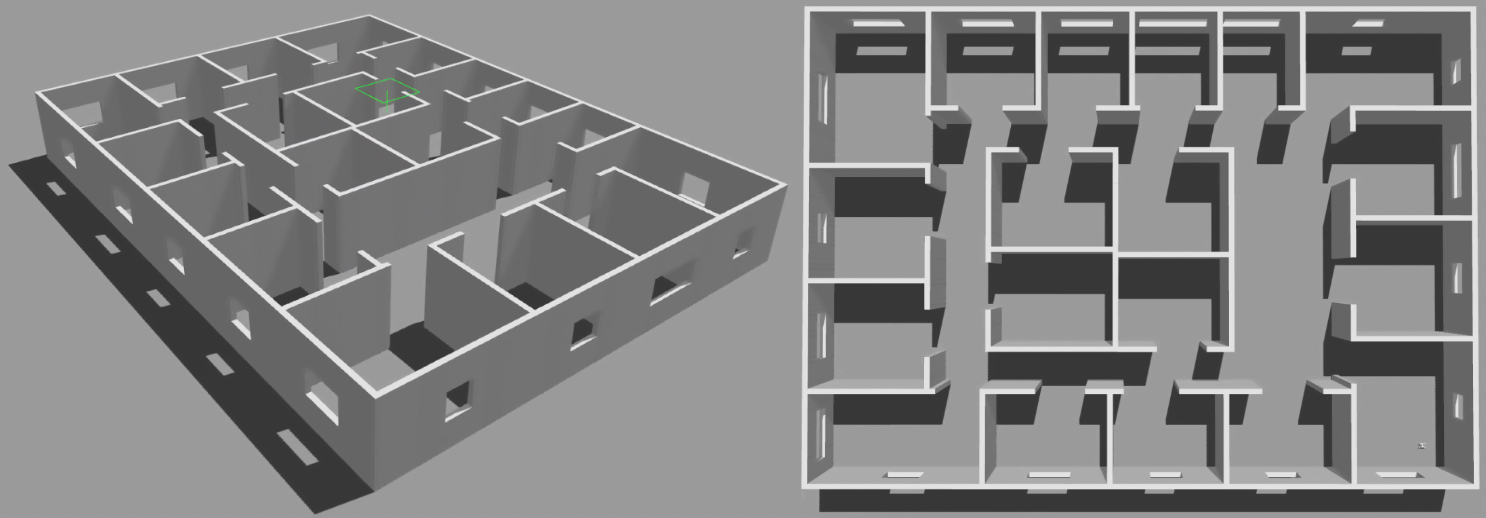
\includegraphics[width=1.0\columnwidth]{fig/sim_env.png}
    \caption{Example of simulation environments,}
    \label{fig:sim_env}
\end{figure}

Besides, we have integrated a customized sonar model into the description file of the dragon ddk drone model. Drawing upon the gazebo range sensor plugin, we have established a series of parameters to accurately reflect the specifications of our actual sonar hardware. This includes variables such as update rate, maximum sensor range, and \glspl{fov}. As the range sensor plugin detects obstacles based on collision properties of the material, we have designed the window material in such a way that it remains detectable to the sonar model. The resulting simulation enables us to replicate various real-world scenarios, such as the drone's encounter with a window, as depicted in the left figure. In this case, the occupancy map, maintained by the depth camera point clouds, does not mark the window area as an obstacle. However, the sonar sensor provides accurate distance measurements to the window, which is visualized as a dark cone originating from the drone.

\begin{figure}[h]
    \centering
    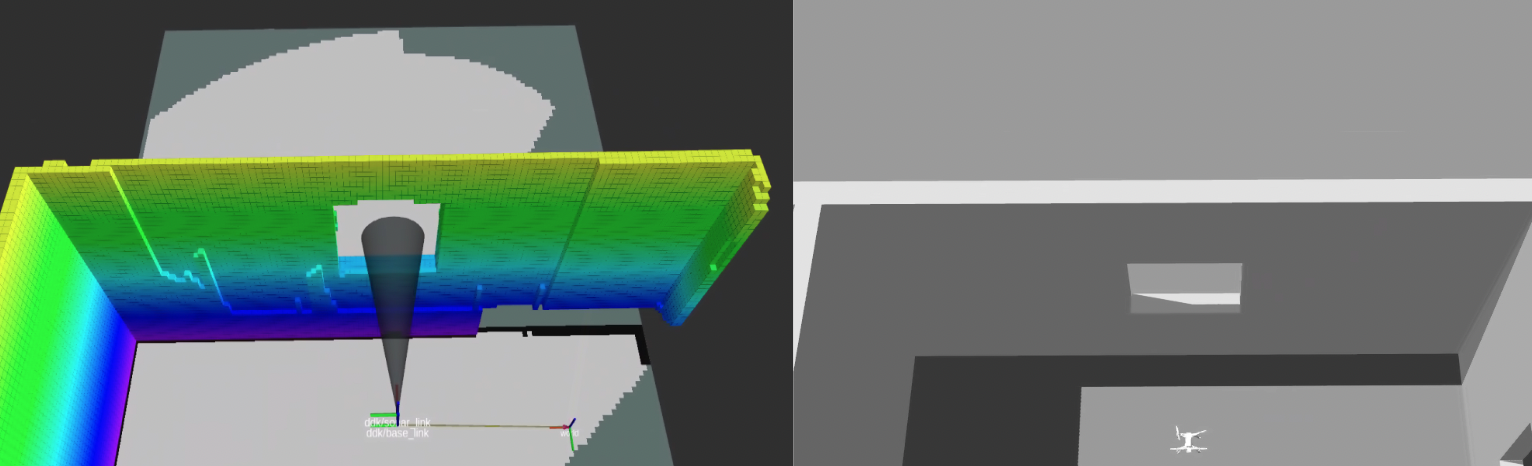
\includegraphics[width=1.0\columnwidth]{fig/sim_sonar.png}
    \caption{Simulated sonar feedback. The right figure shows the drone (white) is facing a wall with a small window in Gazebo simulation. The left figure shows the depth-camera-based occupancy map and the simulated sonar feedback (black cone).}
    \label{fig:sim_sonar}
\end{figure}

\subsection{Inverse Sensor Model}
\label{sec:method_model}
The adaptation of the 3D sonar sensor model stems from the 2D model proposed in \cite{wideanglesonar}. The model accounts for both empty and occupied regions, taking into consideration the range and direction of the grids within the sonar beam. Fig. \ref{fig:sim_sonar_2d}  from \cite{advanced_sonar_sensor} presents a clear representation of a 2D sector of a 3D sonar beam, where the X-axis denotes the direction towards which the sonar sensor is pointing (referred as sonar beam center). The figure corresponds to a sonar beam having a \gls{fov} of $\omega_i$ and a range measurement of $z_i$.

Given a point $p_i$ within the sonar beam and situated at a distance of $r_i$ meters away from the sonar sensor, connecting $p_i$ to the sonar results in a line that forms an angle of $\theta_i$ with the sonar beam center.

\begin{figure}[h]
    \centering
    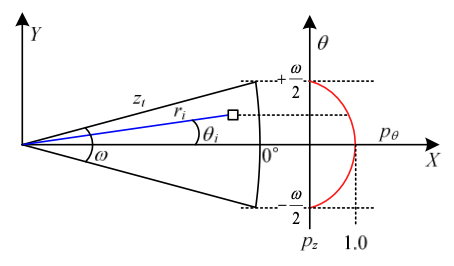
\includegraphics[width=0.5\columnwidth]{fig/sonar_model_2d.png}
    \caption{2D sector of a sonar beam}
    \label{fig:sim_sonar_2d}
\end{figure}

First, we derived a decay term based on $\theta_i$, which is distributed in a semicircular shape as shown in the right-hand side of Fig. \ref{fig:sim_sonar_2d}. The decay term $\alpha_i$ is formulated as:
\begin{equation}
    \alpha_{i} = 1 - (\frac{2 * \theta_i}{\omega})^2
\end{equation}

For a ray of angle $\theta_i$, we compute a decayed $p_{\text{hit}_i}^{\prime}$ and a decayed $p_{\text{miss}_i}^{\prime}$ as below, where $p_{\text{hit}}$ and $p_{\text{miss}}$ is a predefined constant (which is set to 0.7 and 0.3 respectively):
\begin{equation}
    \begin{split}
    p_{\text{hit}_i}^{\prime} = 0.5 + (p_{\text{hit}} - 0.5) * \alpha_{i} \\
    p_{\text{miss}_i}^{\prime} = 0.5 - (0.5 - p_{\text{miss}}) * \alpha_{i}
    \end{split}
\end{equation}

Finally, the occupancy probability of $p_i$ is formulated as follows, where $\epsilon$ is a predefined constant that reflects the expected accuracy of the sonar sensor (which is set to 0.05):
\begin{equation}
    p_{p_i} =
    \begin{cases}
      p_{\text{miss}_i}^{\prime} + (\frac{r_i}{z_i- \epsilon})^2(0.5 - p_{\text{miss}_i}^{\prime}) & \hspace{-3pt}\text{if $r_i \leq z_i- \epsilon$} \\
      p_{\text{hit}_i}^{\prime} - (\frac{r_i - z_i}{\epsilon})^2(p_{\text{hit}_i}^{\prime} - 0.5) & \hspace{-3pt}\text{if $|r_i - z_i| < \epsilon$}
    \end{cases}
\end{equation}

For a better grasp of the sonar model, we have presented a visualization of the occupancy probability along four rays that vary in angles with the sonar beam center in Fig. \ref{fig:sim_sonar_plot}.
\begin{figure}[h]
    \centering
    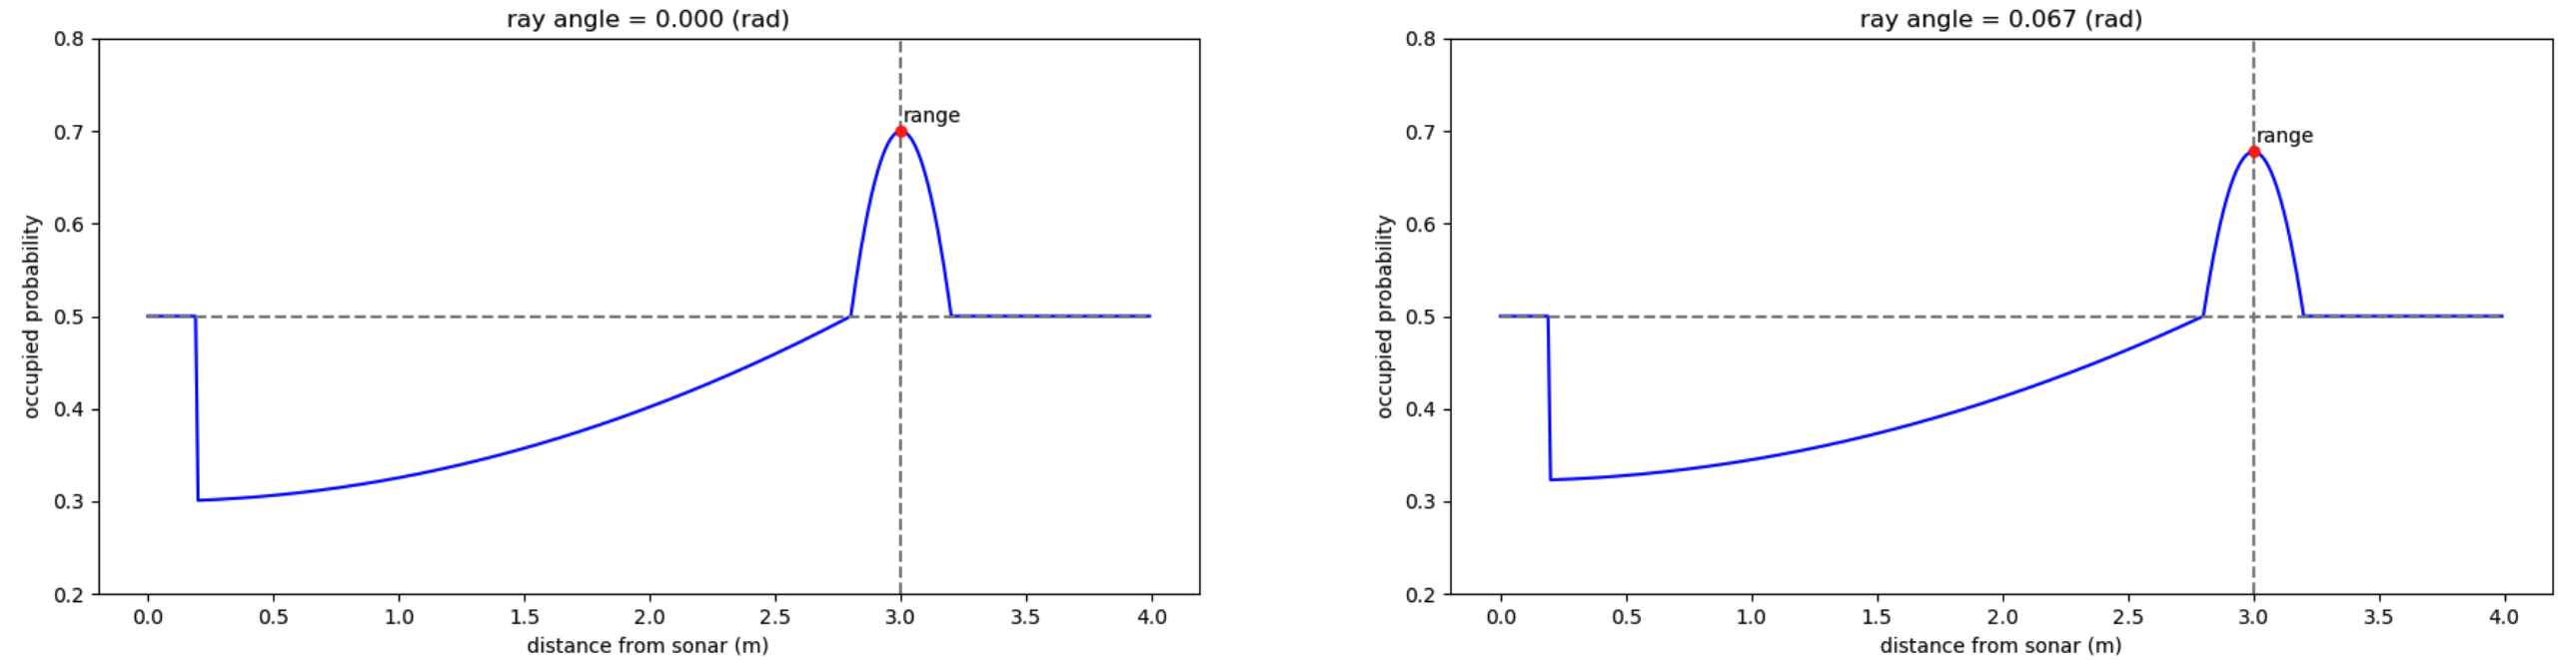
\includegraphics[width=1.0\columnwidth]{fig/sonar_model_1.png}
    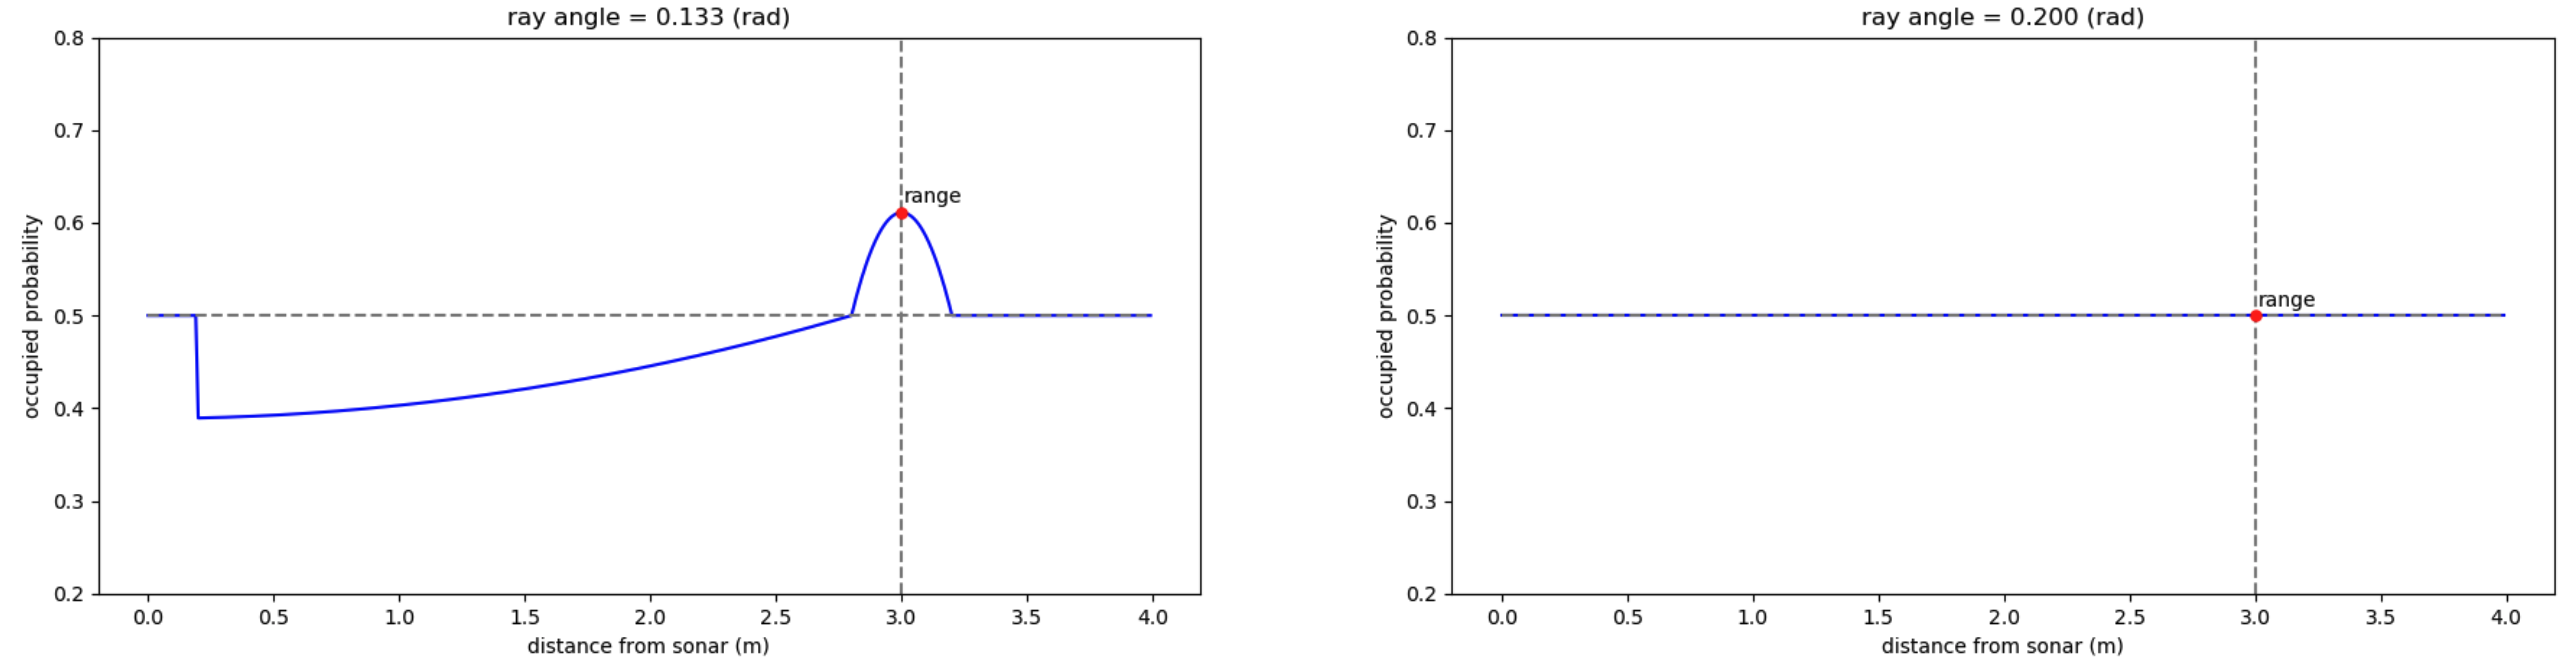
\includegraphics[width=1.0\columnwidth]{fig/sonar_model_2.png}
    \caption{Sonar Inverse Sensor Model Examples: occupancy probability along rays that have different angles with sonar beam center, notice that the sonar \gls{fov} is set the 0.4 rad.}
    \label{fig:sim_sonar_plot}
\end{figure}

As illustrated by Fig. \ref{fig:sim_sonar_plot}, we are more confident with the occupied condition along rays that have smaller angles with the sonar beam center, hence the occupancy probability is updated more confidently. Conversely, the occupied condition near the edge of the sonar beam is less certain, resulting in a more conservative update of the occupancy probability.

\subsection{Sonar Beam Discretization}
\label{sec:method_dis}
Unlike depth images, sonar readings are only scalar values. In order to update the probability of each relevant grid cell in the occupancy map, we need an effective way to discretize the sonar beam.

To address this, we chose to discretize the bottom surface of the spherical cone into dense equidistributed points. This enables us to use the classic ray tracing algorithm \cite{raytracing} to traverse all the grid cells that lie within the sonar beam.

To begin with, a point on the spherical surface can be represented using the classical spherical coordinates, in which a point is addressed via the polar angle $\theta$ and the azimuthal angle $\phi$. If the sphere has a radius $r$, the Cartesian coordinates of that point are given by:
\begin{equation}
    \label{eq:point}
    \begin{pmatrix}
    X \\ Y \\ Z
    \end{pmatrix} = 
    r 
    \begin{pmatrix}
    sin\theta cos\phi\\
    sin\theta sin\phi\\
    cos\phi
    \end{pmatrix}
\end{equation}

The discretization of the spherical cap of our interest is based on the approach proposed in \cite{equidist}, with modifications. In Algorithm~\ref{alg:equidist}, $N$ represents the desired number of points, and $\omega$ represents the \gls{fov} of the sonar sensor. To achieve a nearly regular equidistribution, we first choose circles of latitude at constant intervals $d_{\theta}$, and then on these circles, we choose points at constant intervals $d_{\phi}$. The selection of $d_{\theta}$ and $d_{\phi}$ is made to satisfy the condition $d_{\theta} \approx d_{\phi}$.

\begin{figure}[t]
\begin{algorithm}[H]
\scriptsize
\captionsetup{font=scriptsize} % set size of caption font
\caption{Generate equidistributed points on the spherical cap}\label{alg:equidist}
\begin{algorithmic} [1]
\State $a \gets$ $4\pi / N$;
\State $M_{\theta} \gets \lceil \pi / \sqrt{a} \rceil$;
\State $d_{\theta} \gets \pi / M_{\theta}$;
\State $d_{\phi} \gets a / d_{\theta}$;
\For{each $m$ in $0, ..., M_{\theta} - 1$}
\State $\theta \gets$ $\pi (m + 0.5) / M_{\theta}$;
\If{$\theta > \omega$ / 2}
    \State break;
\EndIf
\State $M_{\phi} \gets \lceil 2\pi sin\theta/ d_{\phi} \rceil$;
    \For{each $n$ in $0, ..., M_{\phi} - 1$}
        \State $\phi \gets$ $2\pi n / M_{\phi}$;
        \State create a point using Eq. \ref{eq:point}
    \EndFor
\EndFor
\end{algorithmic}
\end{algorithm}
\vspace{-1cm}
\end{figure}

\subsection{Occupancy Map Update}
\label{sec:method_occ}
To maintain an accurate and comprehensive representation of the surrounding environment, we maintained two separate occupancy maps. The first occupancy map is created solely using depth camera data, which provides reliable and precise information about the environment. The second occupancy map is updated with sonar readings, which can detect objects that are not visible to the camera.

To update the sonar occupancy map, we use the classic ray tracing algorithm, accompanied by the sonar's \gls{ism} and beam discretization method described in previous sections. However, not all sonar readings are accurate or informative, so we filter the readings based on their correspondence with the depth camera data. We consider three cases of sonar and depth camera correspondence. In case (a), the camera layer marks multiple cells inside the sonar beam as occupied, we assume that both sensors detected the same object, and we discard the sonar data. In case (b), the camera layer marks multiple cells inside the free space of the sonar beam as occupied, we assume that the sonar measurement is incorrect, and we discard the sonar data. In case (c), the camera does not detect anything, while the sonar receives reflections from objects within its sensing range, we suspect that there may be a glass wall in front of the robot. In this case, we update the sonar occupancy map with the current sonar reading.

\begin{figure}[h]
    \centering
    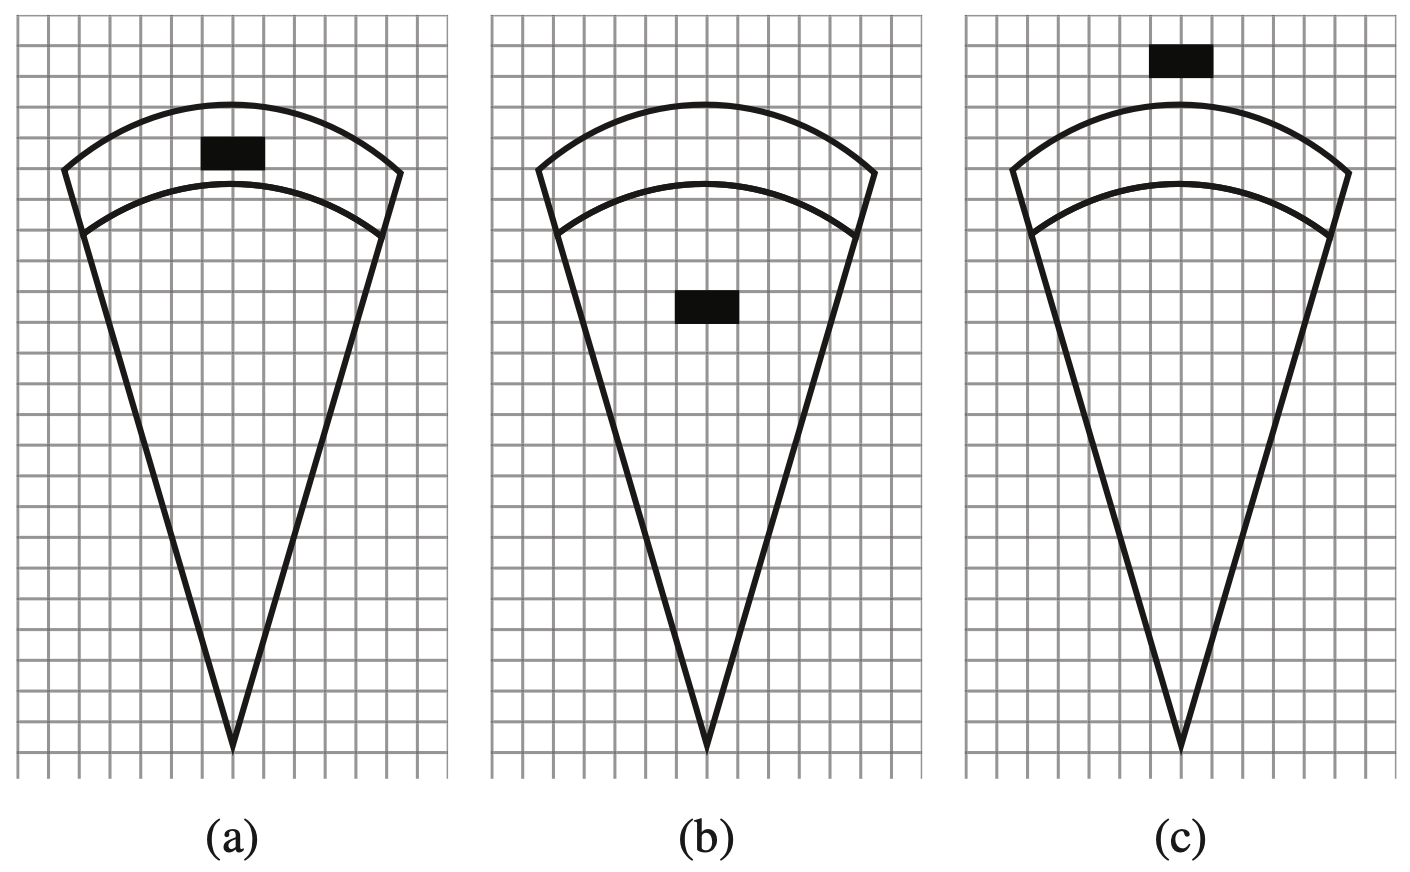
\includegraphics[width=0.8\columnwidth]{fig/occ.png}
    \caption{Three Cases of Sonar-Depth Correspondence.}
    \label{fig:occ}
\end{figure}

We illustrate these three cases in 2D space in Fig. \ref{fig:occ} from \cite{camerafusion}, where the underlying grid represents the current occupancy map created solely by the depth camera. Black cells represent objects, and white cells represent free space. The sonar beam is visualized and divided into two parts, with the lower part representing free space and the upper part representing the region where the sonar detects objects. The flow chart in Fig. \ref{fig:occ_flow} visualizes the mechanism described above.

\begin{figure}[h]
    \centering
    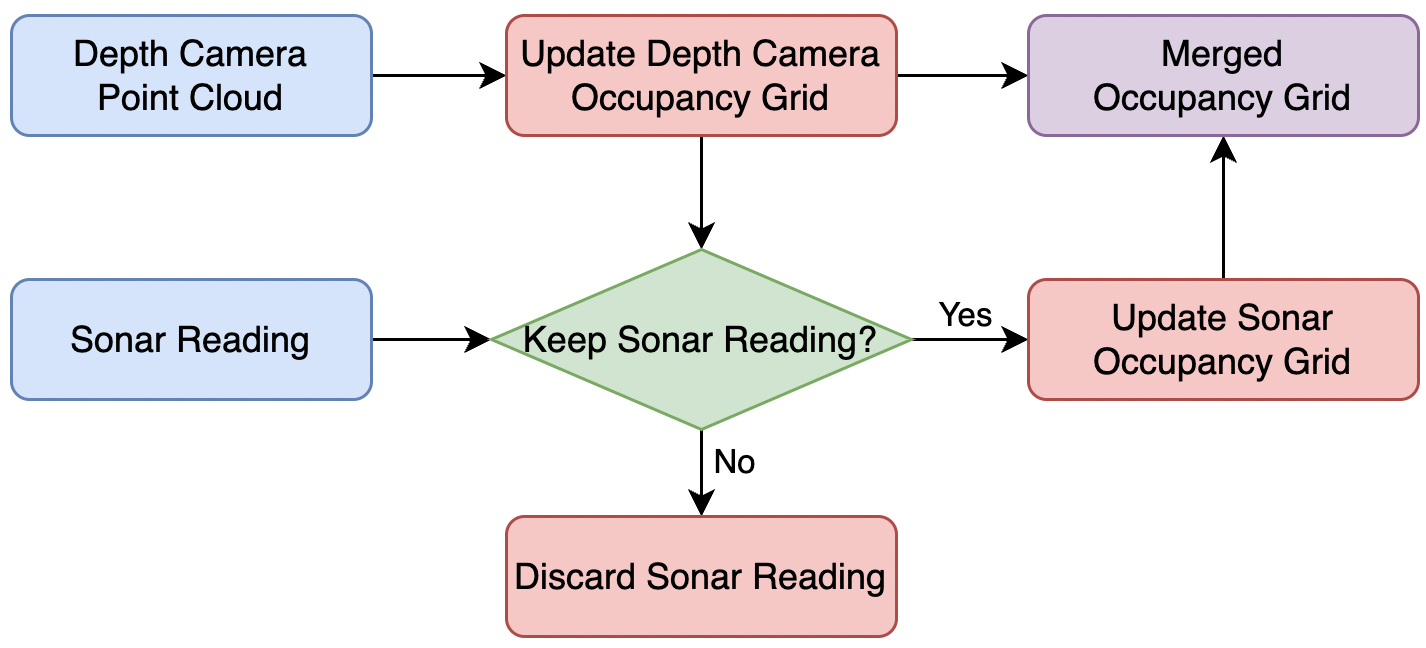
\includegraphics[width=0.8\columnwidth]{fig/occ_flow.png}
    \caption{Flow chart of occupancy map update.}
    \label{fig:occ_flow}
\end{figure}

To demonstrate the effectiveness of our approach, we compare the occupancy map built solely using depth images with the occupancy map maintained by fusing depth images and sonar readings in Fig. \ref{fig:occ_comp}. We observe that the depth-images-only map fails to mark the center region of the wall as occupied, which corresponds to a simulated glass window. In contrast, the merged map successfully marks the glass region as occupied based on sonar readings while retaining accurate information on the other parts of the environment provided by depth images.

\begin{figure}[h]
    \centering
    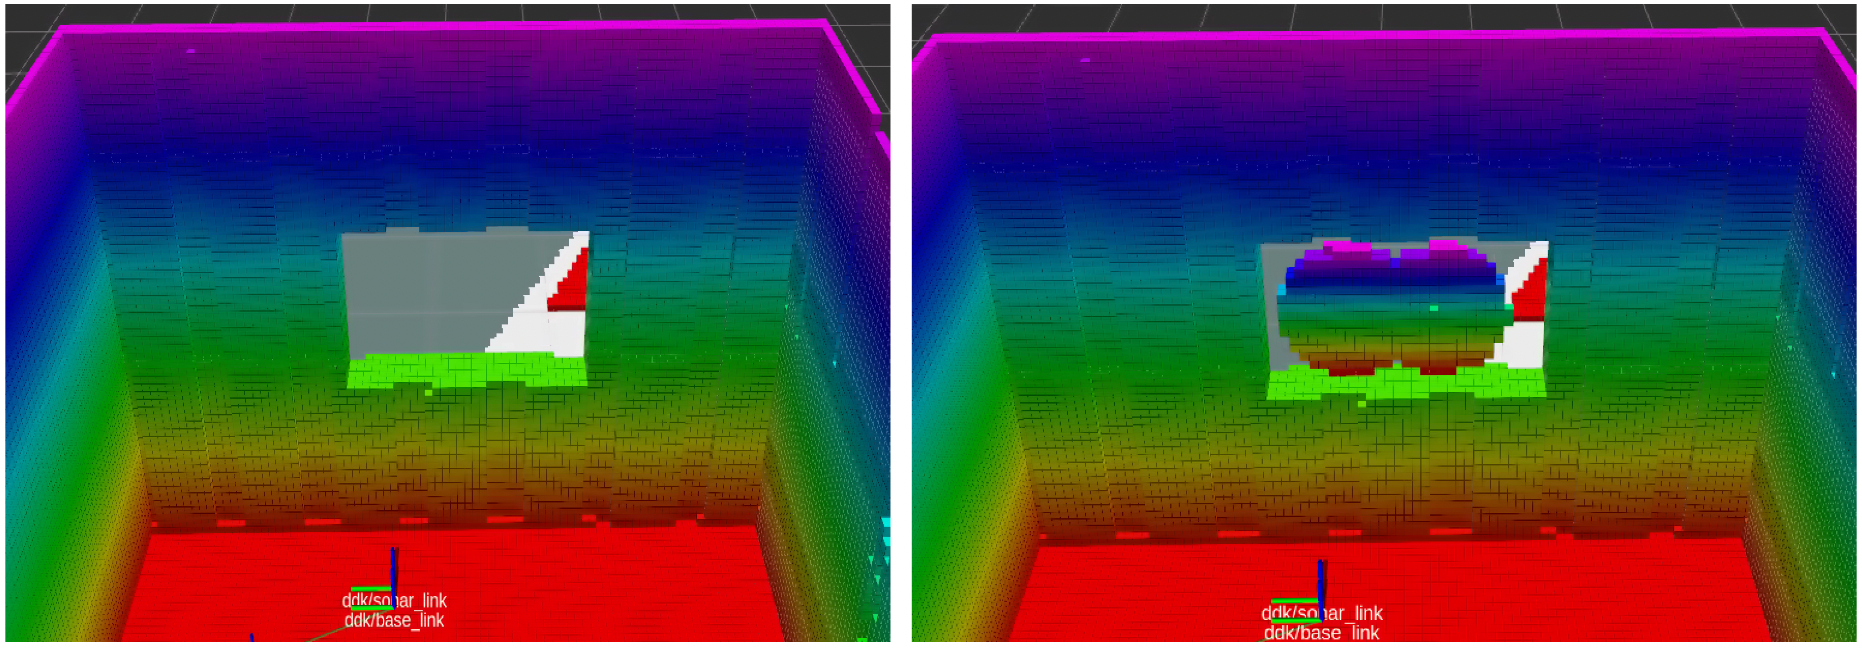
\includegraphics[width=1\columnwidth]{fig/occ_comp.png}
    \caption{Map built on depth images vs. sonar readings \& depth images.}
    \label{fig:occ_comp}
\end{figure}

\subsection{RANSAC-based Window Segmentation}
\label{sec:method_ransac}
In certain scenarios, particularly in indoor exploration, it is advantageous to have semantic knowledge about the location of windows. Such information may enhance the efficiency of exploration logistics. In this study, we propose a RANSAC-based approach for window segmentation. The method initially identifies the region of interest based on the discrepancy between the sonar reading and the depth-image-based occupancy map. Then, the potential location of the window is further determined by its geometric characteristics. The flowchart illustrated in Fig. \ref{fig:ransac_flow} depicts the mechanism.

\begin{figure}[h]
    \centering
    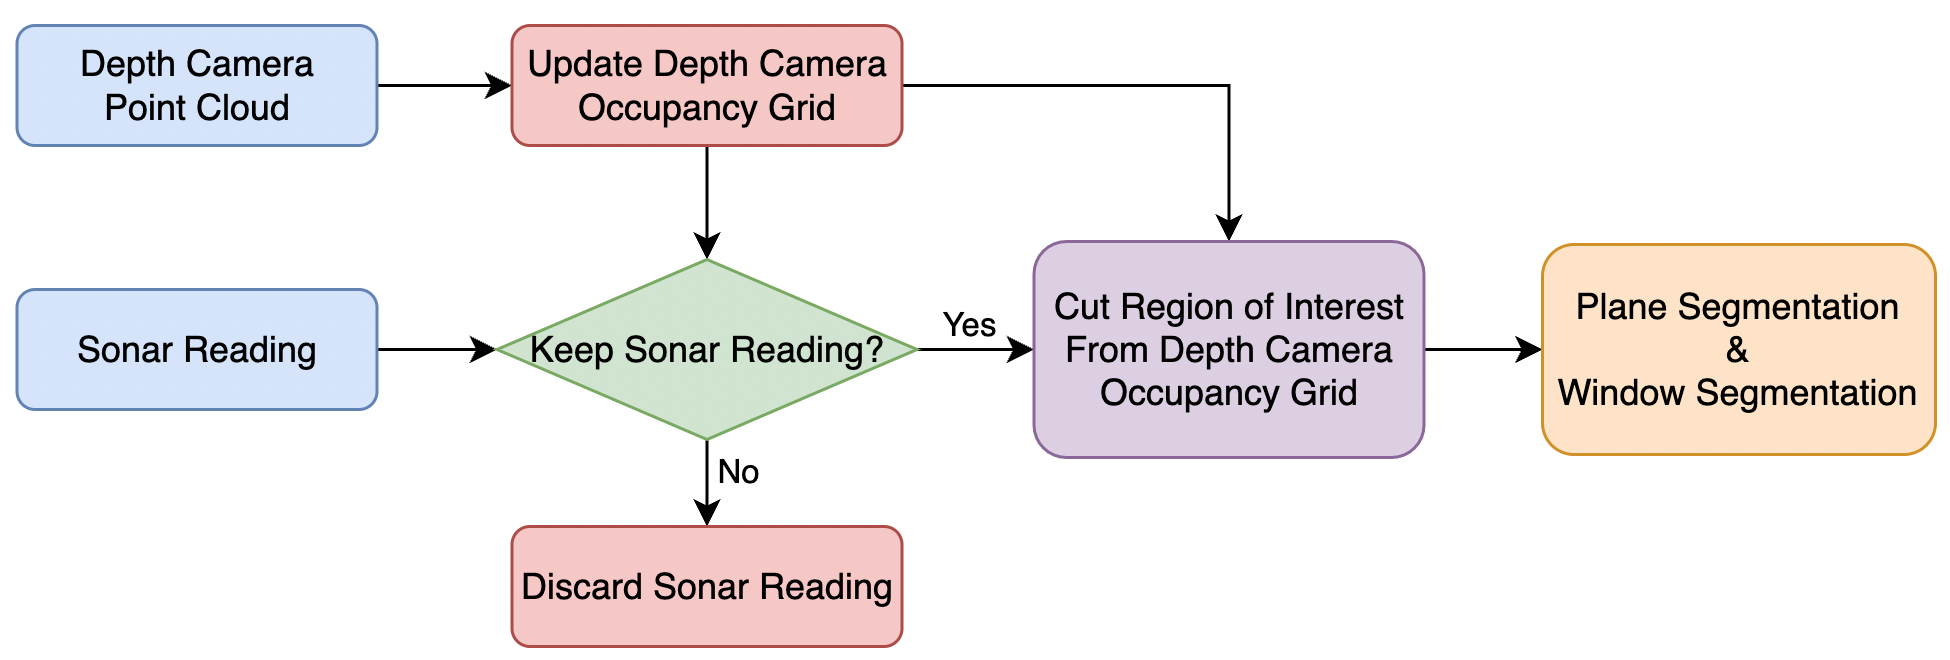
\includegraphics[width=1\columnwidth]{fig/ransac_flow.png}
    \caption{Flow chart of RANSAC-based Window Segmentation.}
    \label{fig:ransac_flow}
\end{figure}

As seen from Fig. \ref{fig:ransac_flow}, the segmentation process's initial stage is precisely the same as the occupancy map update pipeline. The sonar reading that contains valuable information is determined first. Since the sonar reading is retained only when it detects potential obstacles that are not detected by the depth camera, a window is likely to exist in the sonar reading's vicinity. Therefore, we consider the center point of the sonar reading (i.e., the center of the sonar beam's bottom surface) as the pivot and extract a region of interest in the size of a 5-meter by 5-meter box with a height of 3 meters.

Next, we utilize the SACSegmentation pipeline, which is supported by the PCL library, to segment the largest plane in the region of interest. If the magnitude of the $z$ coefficient of the fitted plane is below a certain threshold (e.g., 0.01), the plane is nearly vertical to the ground plane, which indicates that it is highly likely to represent a straight wall in an indoor environment. In the left-hand side of Fig. \ref{fig:ransac}, an example of fitted vertical planes can be seen. The white regions represent all inlier grid cells. However, due to simulated sensor noise, the occupancy representation of a flat wall may not appear completely flat. As a result, there may be several vertical gaps among white regions.

The final stage involves searching along the fitted plane for any rectangular openings, which represent the potential window region. The occupancy grid provides us with a discretized representation of the fitted plane, allowing us to search the plane vertically line by line. For each line, we count the number of unoccupied cells. Finally, we consider the region framed by vertical lines that contain a similar number of free-space cells as the potential glass region.

\begin{figure}[h]
    \centering
    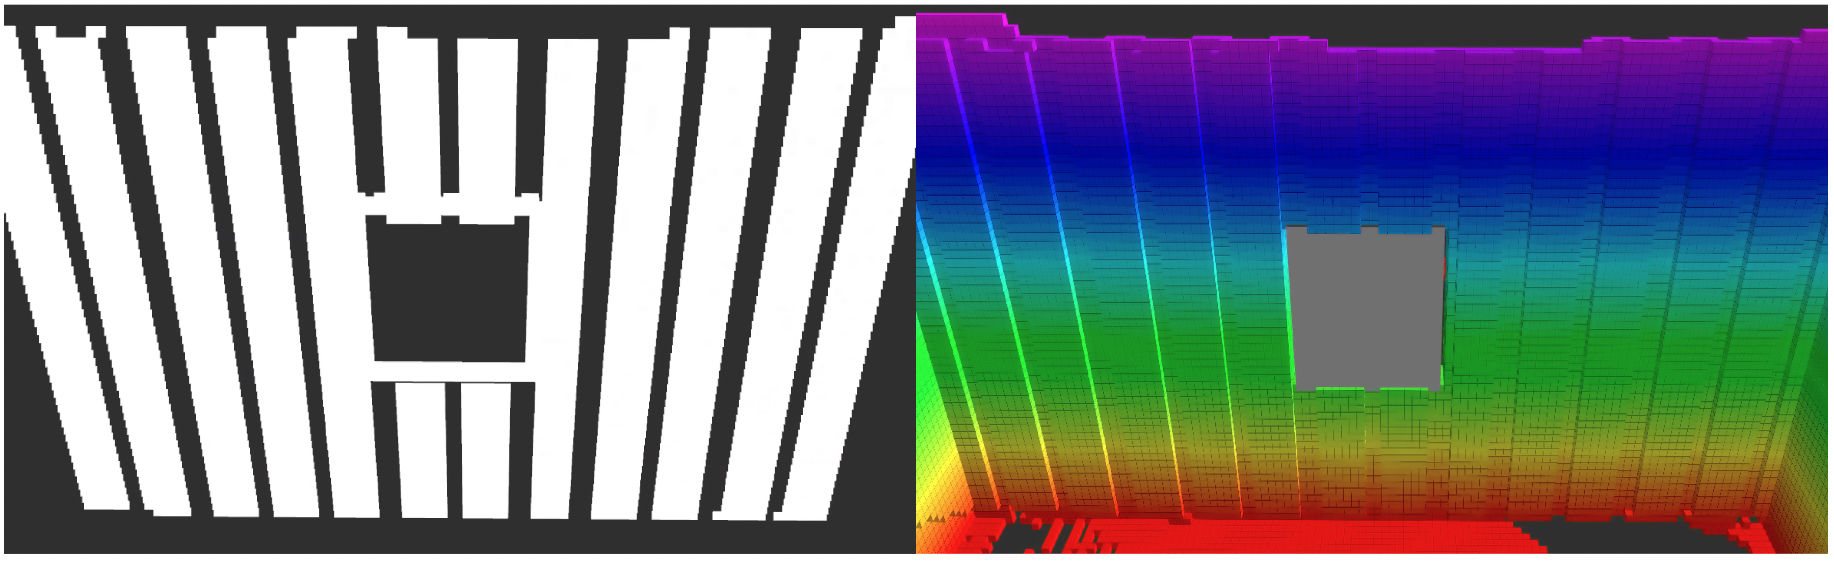
\includegraphics[width=1\columnwidth]{fig/ransac.png}
    \caption{RANSAC-based Window Detection. The left image displays all the inliers on the fitted largest plane. The right image depicts the occupancy map, with the window segmentation marked in grey.}
    \label{fig:ransac}
\end{figure}

The right-hand side of Fig. \ref{fig:ransac} shows an example of the segmented window area, which is marked in grey and framed by the colorful depth-camera-based occupancy grids.